% Straight up stealing preamble from Eli Holmes 
%%%%%%%%%%%%%%%%%%%%%%%%%%%%%%%%%%%%%%START PREAMBLE THAT IS THE SAME FOR ALL EXAMPLES
\documentclass{article}

%Required: You must have these
\usepackage{Sweave}
\usepackage{graphicx}
\usepackage{tabularx}
\usepackage{hyperref}
\usepackage{natbib}
%\usepackage[backend=bibtex]{biblatex}
%Strongly recommended
  %put your figures in one place
 
%you'll want these for pretty captioning
\usepackage[small]{caption}

\setkeys{Gin}{width=0.8\textwidth}  %make the figs 50 perc textwidth
\setlength{\captionmargin}{30pt}
\setlength{\abovecaptionskip}{0pt}
\setlength{\belowcaptionskip}{10pt}
% manual for caption  http://www.dd.chalmers.se/latex/Docs/PDF/caption.pdf

%Optional: I like to muck with my margins and spacing in ways that LaTeX frowns on
%Here's how to do that
 \topmargin -1.5cm        
 \oddsidemargin -0.04cm   
 \evensidemargin -0.04cm  % same as oddsidemargin but for left-hand pages
 \textwidth 16.59cm
 \textheight 21.94cm 
 %\pagestyle{empty}       % Uncomment if don't want page numbers
 \parskip 7.2pt           % sets spacing between paragraphs
 %\renewcommand{\baselinestretch}{1.5} 	% Uncomment for 1.5 spacing between lines
\parindent 0pt% sets leading space for paragraphs
\usepackage{setspace}
%\doublespacing

%Optional: I like fancy headers
\usepackage{fancyhdr}
\pagestyle{fancy}
\fancyhead[LO]{How do climate change experiments actually change climate}
\fancyhead[RO]{2016}
 
%%%%%%%%%%%%%%%%%%%%%%%%%%%%%%%%%%%%%%END PREAMBLE THAT IS THE SAME FOR ALL EXAMPLES

%Start of the document
\begin{document}

% \SweaveOpts{concordance=TRUE}
 \bibliographystyle{/Users/aileneettinger/citations/Bibtex/styles/nature.bst}
\title{How do climate change experiments actually change climate?} % Paper 1/Large group paper from Reconciling Experimental and Observational Approaches for Climate Change Impacts

\author{A.K. Ettinger,I. Chuine, B. Cook, J. Dukes, A.M. Ellison, M.R. Johnston, A.M. Panetta,\\ C. Rollinson, Y. Vitasse, E. Wolkovich}
%\date{\today}
\maketitle  %put the fancy title on
%\tableofcontents      %add a table of contents
%\clearpage
%%%%%%%%%%%%%%%%%%%%%%%%%%%%%%%%%%%%%%%%%%%%%%%%%%%

\section* {Aim}

The aim is to write a Concept/Synthesis Paper, for Nature Climate Change, about maximizing benefits of field-based climate change experiments. We argue that there is a need to improve our understanding of how climate is actually altered by these experiments, particularly if we wish to use these experiments to forecast biological impacts of climate change. %yann: perhaps also to determine which methods of warming alter the least other climatic variables or to define the most appropriate method regarding the focus of the study (phenology, growth, survival etc)?%annmarie: Somewhere in this paper,  we should discuss that is important that “how” climate variables are modified relative to the predicted change under various emission scenarios is important.  Thus, the “how” should be not only the direction and magnitude of the variable change but also the extent to which the change mirrors change projected for the region in which the experiment took place). build up a discussion of studies that report only mean shifts in temperature in the intro.

\section* {Introduction}
% EMW: Some changes below -- tried to break up the two long, complicated sentences. I think we also need a little more intro to climate change here and acknowledgment that it IS already changing. Adjust so it reads more like: climate change is shifting things, future change will be even bigger with cascading effects...
\par Ongoing climatic changes are causing dramatic alterations to Earth's biota, increasingly altering the physiology, distribution, and abundance of organisms that result cascading community and ecosystem effects \citep{thomas2004,parmesan2006,sheldon2011,urban2012}.  Much uncertainty remains, however, about how particular individuals, populations, species, communities, and ecosystems will respond as changes become more extreme. Predicting these biological responses to current and future climate change, as well as they will feedback to affect earth's climate and ecosystem services, are among the most significant challenges facing biologists today.
% EMW: See quick (could be much better) changes below to better handle temperature and precipitation in this paragraph. Much work is on temperature because that's a known, relatively easy to predict effect, at least when compared to precipitation (we may or may not want to sneak this in). Mirriam suggests adding these citations:> Charney 1975. Dynamics of deserts and droughts in the Sahel. Quarterly Journal of the Royal Meteorological Society 101, 193-202. 
% Shukla and Mintz 1982. Influence of land surface evapo-transpiration on the Earth's climate. Science 25: 1498-1501.
%Cox et al. 2000. Acceleration of global warming due to carbon-cycle feedbacks in a coupled climate model. Nature 408: 184-187.
% Field et al. 2007. Feedbacks of terrestrial ecosystems to climate change. Annual Review of Environment and Resources 32: 1-29.

\par Researchers have sought to understand and forecast biological responses through a variety of approaches, including observational studies, model-based approaches, and experiments. Observational studies typically correlate observed biological patterns with trends in climate; however, it is challenging to disentangle the causal effect of warming from other factors that have also changed, such as land-use change. In addition, future climate change is expected to result in conditions that are outside those that have been observed historically \citep{ohlemuller2006,williams2007,williams2007b,ipcc2013}. Modelling techniques can be useful in this regard, but these methods often rely on untested assumptions, for example, that climate limits performance \citep{pearson2004,ibanez2006,swab2012}. Experiments are therefore a critical component of the biologist's toolkit for understanding climate change impacts, and are often considered the "gold standard" of knowledge \citep[e.g.][]{box1978,gelman2014}. In situ climate warming experiments allow effects of temperature and  precipitation to be isolated from other  environmental changes that can confound conclusions drawn from observational data sets. In addition, a range of warming  and/or precipitation treatments can be applied, such that potential non-linear responses can be evaluated. Compared with controlled growth-chamber experiments, field-based experiments offer the possibility of preserving important, but unknown or unquantified, in situ biotic and abiotic drivers and interactions. Climate change experiments in the field may therefore be able to illucidate many biological responses to future climate change.
\par Experimental climate manipulations take a variety of forms, manipulating temperature, precipitation, atmospheric CO2, and other variables using a wide range of techniques \citep{shaver2000,aronson2009}. In the field, temperature increases can be simulated using "passive" warming infrastructure, such as open-top chambers, that trap energy already available in the environment or "active" warming methods, which heat ecosystems using external energy inputs (e.g., gas-powered forced air heaters, electrical-powered soil warming cables and/or infrared heaters \citep{shaver2000}. Many field experiments have explored biological responses to interacting environmental changes: active warming methods have been combined with  precipitation manipulations, (e.g. snow removal,  water additions and reductions), in  an  effort to create  climatic  conditions such  as  those  forecasted  under  future climate  change scenarios \citep{price1998,cleland2006,sherry2007,rollinson2012}.
\par In this synthesis, we focus on in situ active warming  manipulations, for they offer several advantages over both passive warming methods and other approaches that rely on long-term observational data and growth chamber manipulations.  Recent analyses indicate that active warming methods are the most controlled, consistent, and "true to climate change predictions" \citep{kimball2005,kimball2008,aronson2009,wolkovich2012}. These advantages come at a cost, however.  Experimental in situ active climate  manipulations are logistically challenging  and expensive; it is difficult to design,  implement,  and  monitor  replicated experiments that consistently apply  the intended climate  manipulations \citep{aronson2009}.
\par Seeking to prepare  for future, altered  biological conditions, scientists and others  often attempt to extrapolate the results of in situ climate change experiments to forecast how organisms and ecosystems will respond to particular climate change scenarios.  Even in cases where extrapolation is not the explicit goal of climate change experiments, these studies are often used to draw conclusions  about how anthropogenic warming  will affect species' performance  (e.g. growth and  survival)  and  distributions (WE MAY WANT SOME CITATIONS HERE).  Despite this tendancy, a detailed  assessment of how different types of experimental warming technologies actually alter environmental conditions experienced by the organisms, and  the extent to which these conditions simulate anticipated climate change, is lacking.  
\par In this synthesis, we first use  plot-level daily  microclimate  data  from  12 climate  change  experiments  that  manipulate temperature and precipitation, in some cases, to demonstrate the direct and indirect ways in which environmental conditions are altered  by active  warming technologies.   The data we use were collected between 1991 and 2014 from North American and European climate change experiments and  have been merged into a new, publicly  available  database (see Supplemental Materials  for details).   We then highlight the challenges that each of the technologies create for interpreting biological responses to climate manipulations and using these interpretations to forecast  more widespread responses to contemporary climate change. Finally,  we use findings from our synthesis to make recommendations for future  climate  change experiments.

%In addition, a range of warming and/or precipitation treatments can be applied, such that potential non-linear relationships of climate responses can be evaluated. These advantages come at a cost, however. The most accurate experimental in situ climate manipulations (i.e., active warming methods) are logistically challenging and expensive \citep{aronson2009}. Even with extensive resources it is often difficult to design, implement, and monitor replicated experiments that consistently apply the intended climate manipulations. Yet, despite these limitations, field warming experiments offer some of our best estimates of future biological responses to warming. 

%\par Given warming experiments' high value in estimating ecological responses scientists and others often wish to extrapolate the results of in situ climate change experiments to forecast how organisms and ecosystems will respond to particular climate change scenarios. Even in cases where this is not the explicit goal of warming and other climate change experiments, it would be incredibly useful to be able to apply knowledge gained from these experiments to improve our understanding and forecasting of how anthropogenic warming will affect species' performance (growth, survival) and distributions. Our ability to make this application, however, is currently limited. This is because we lack a detailed assessment of exactly how experimental warming treatments alter climate and the extent to which these manipulations accurately model the real world, both present and future. 
% CRR: Maybe add something here or somewhwere else in the intro about this might be important for reconciling experimental results with each other as well as with observational studies?
%\par To realize the forecasting potential of climate change experiments, a more nuanced understanding of how climate change experiments actually change climate is critical. Towards this goal we carried out a full literature review to identify all active field warming experiments then obtained daily (or sub-daily) climate data from as many as possible (we obtained data for 12/XX total identified experiments, see Supplemental Materials for details). We are thus able to show, for the first time, the complex ways that climate is altered by active warming treatments, both directly and indirectly. The data we use are from experiments in North America and Europe that were collected between 1991 and 2014, and have been merged into a new, publicly available database (names GOOBER). We then discuss the challenges of interpreting biological implications of experimental shifts in climate, when these climate manipulations are more complex than simple shifts in the mean. Finally, we make recommendations for future climate change experiments.
% Need to give the database a name!

\section* {Complications in extrapolating experimental climate change}
Climate change experiments often include detailed monitoring of climate variables at the plot level, yielding large amounts of data, such as daily or hourly temperature and other climate variables, over the course of the experiment. However, biologists are generally interested primarily in the biological responses associated with each treatment (e.g. growth, abundance, or phenology of a species). Not surprisingly, then, authors typically provide detailed information on the observed biological responses, and report only the mean change in climate over the course of the experiment and whether or not that mean change matched their target level of change \citep{price1998,clark2014a,clark2014b,rollinson2012}. 
%CRR: I think it's good that you mention we don't report the climate because we're interested in the organisms and it leads to a publication bias.  I don't know how to phrase it, but we (people that did the experiments) also often don't go into more detail because the experimental application can be very buggy with sensors going out, power outages, etc. and we've had to find that balance between accurately reporting our ecological story without going into the endless pits of study caveats.
\par Though the published focus is often on shifts in the mean, the imposed climate manipulations result in much more complex shifts of climate. The magnitude of change experienced by organisms in these manipulations is likely to vary in time and space, and the equipment required to conduct these manipulations can also alter climate at the plot level, perhaps challenging results interpretation. % EMW: Last sentence is a lot here -- can you break into two? One would be on changes to climate and the other can make the leap to organisms.% CRR: Agree with Lizzie -- I'm having a hard time making the jumps -- isn't modifying plot-level climate the purpose?  or are you talking about sham controls? By complex shifts in climate are you talking about the weird diurnal/seasonal patterns, weird above- & belowground relationships among temp & moisture?


\subsection* {Treatments vary over time}
The common practice of reporting only the mean temperature difference, across the duration of the study, may hide variations in annual, seasonal, and daily minimum and maximum temperatures.There are frequently strong seasonal variations in experimental warming effects (Figure 1). %Yann: so this is due to interactions between the artificial treatment with natural climate variation.
%Miriam: •	To me, Figure 1 doesn't show “strong seasonal variations in experimental warming effects” [maybe Figure #s in text and on figures don't correspond right now? That happens to me all the time :-)]. Block is a spatial thing, and it would be great to add time frequencies to augment “by year.” Here are some possibilities for plots to show treatment variation over time:
%	Yearly: year on x axis, deviation from target warming on y axis, experiments coded by shape
%	Seasonally: season on x axis, deviation from target warming on y axis, experiments coded by shape
%Between days: Pick a representative year, put DOY on the x axis, deviation from target warming on the y axis, experiments coded by shape
%Within days: Pick a representative year, put DOY on x axis, (max temp – min temp) on the y axis, experiments coded by shape
%Figure 2 is only one year (?), so it doesn't show treatments varying “among years”
%The rainstorms idea is interesting and seems potentially relevant at several time scales, but probably most relevant at the shorter timescales (daily or monthly?). 
%	Structurally, this section would flow best if it went from slow to fast or from fast to slow (i.e. yearly > seasonally > daily > within days, or the opposite).
%	“...comparison of projections versus observations in climate change experiments is lacking” – does this mean targets vs. observations? “Projection” sounds like a model output to me. 
% CRR: I think Marhsall McDaniel published some stuff from our experiment to support Yann's poing.
This can occur because treatments are not applied consistently over the year, either because heat applications are frequently shut off during some seasons such as when snow cover is present \citep[e.g.][]{clark2014a,clark2014b,hagedorn2010} or because some heating methods, even if left on throughout the year, are not capable of applying consistent warming year-round (e.g. infrared radiation, CITATION- Christy, Yann, and/or Jeff could you suggest 1 or 2?). %Yann: Somewhere we should also say that if not applied all the year around, it is nor realistic because of the plant-soil interactions (microbial communities might be affected by the warming during winter and if it is applied only in summer it is highly artificial and may release much more nutrients that it would do if conducted over the year)
Furthermore, seasonal precipitation patterns can alter the effectiveness of warming treatments (CITATION- Christy, Yann, and/or Jeff could you suggest 1 or 2?). % it is likely that this would yield different effects than if heating were turned on during winter (because then you change soil nutrient mineralization which might be important in winter and so change nutrient availability and moisture for the growing season ).
% EMW: Can you show any of the diurnal changes you mention? At least in the supp?
% CRR: Is this seasonal precip pattern related to the point about snow cover you mention earlier?  I'm wondering if there's some sort of snow or climatic threshold where warming has less of an impact.
\par In addition to seasonal fluctuations, experimental warming effects can vary across years  (Figure  2).   This  can be due  to interactive effects of warming  treatments and  other aspects of weather  that may  vary  annually.  For  example,  Hoeppner  and  Dukes  (2012) found  that infrared heaters  failed to achieve the target temperatures during  rainstorms;%JD: seems like an example of how treatments can vary across hours or days not years...
this has also been observed by Peterjohn et al. \citep{peterjohn1993} for soil warming cables.  %BEn: My turn to be annoying and pedantic! But here I also think you make the point I was trying to make above ("aspects of weather that may vary annually”). At the end of the day, all we can try to do is manipulate the climate, and any weather variations will be imposed on top of this. % CRR: Kimball who did the initial IR heater work also has a long list of caveats in his papers -- wind is also a big one. I think he's the one that cites heater effectiveness & trouble in hot, sunny days where surface temperatures already get really hot as why we had the different levels of heating in day & night. (related to your next point)

\par Warming treatments can also vary on shorter timescales, such as within a day. This often leads to a decrease in the diurnal temperature range within experimental plots, compared with ambient conditions \citep{hoeppner2012}. This may be similar to what is projected for parts of world \citep{ipcc2013}. However, this will likely vary spatially, as some regions have experienced higher daytime warming than nighttime warming, whereas others have experienced the opposite \citep{ipcc2013}. %yann: say why this is very important to know whether warming is more effective during days than during nights for example...recent article that experimentally warmed either during nights or days or both and show that diurnal temperature impact much more phenology than nocturnal temperatures (at equal temperatures).\citep{fu2016}.
% At ESA a couple years ago I saw a guy gave a talk showing how the different day/night warming impacted arthopod communities (they enclosured warming experiments with different diurnal warming patterns).  I wish i remembered the name, but will try to remember to search around for it... I think it was a student/postdoc with Oswald Schmitz (Yale).


\par A detailed comparison of projections versus observations in climate change experiments is lacking. Thus, it is unknown how divergent these annual, seasonal, and daily variations may be from real (i.e. non-experimental) climate patterns.  %there are several recent papers showing the importance of diurnal over nocturnal temperature on phenology. %EMW: Adjust above paragraph to focus also what we need to do. 

\par Anne Marie- please write a paragraph on your suggested discussion "that 3-5 year studies may not capture ultimate, long-term responses that may actually be in the opposite direction to short-term responses.  Cite recent Global Change Biology paper by Harte et al.  Ideally, we want to run studies long enough to capture population-level responses to warming." I would love to work this in and I think you are the one to write it!
%yann:I suggest that warming treatments also buffer extreme cold events. It would be nice to compare for instance minimum temperatures (or absolute minimum temperature) in spring between the control and the warming treatment and to see if this difference is bigger than between the mean or max temperature. I expect it to be much larger during cold night with clear sky due to radiative cooling in the control that is not occuring in the warming plot due to artificial warming...
\subsection* {Treatments vary in space}
In addition to temporal variation, there can be spatial variation in experimental warming effects, such that extrapolation of experimental warming to forecast climate change impacts may not be a straightforward space-for-time substitution. For example, our database contains three studies that used a blocked designs, allowing us to examine spatial variation in the amount of warming (i.e. the difference between treatment and control plots within a block). We found that the amount of warming may vary by more than one degree among blocks (Figure 2, Table 1), resulting in lower warming treatments that varied almost 100\% of their target temperature and higher warming treatments varying 20\% (EMW: I am eye-balling, give exact values).% EMW: I offered one way to build on the finding, you could come up with many others instead -- I think it is important to just point it out a little more. 
%Miriam: •	Figure 2 doesn't explicitly look at blocks•	Is the issue with spatial variation that we can't easily do space-for-time substitution, or is spatial variation simply another symptom that we're not effectively hitting targets?

\par Presumably, there will be spatial variation in future climate change effects, given that warming to date has varied spatially \citep{ipcc2013}).  Accurate extrapolation of climate change experiments may therefore depend on the extent to which experiments encompass a representative amount of existing natural variation (e.g. gradients in slope, aspect, etc) present at the scale at which the extrapolation is being made. 
% CRR: There's some lit out there that talks about the geographical of bias of climate change research... I know some of it is related to flux tower location & I think some papers came out as NEON was getting rollign to justify their geographical approach
\par An added complication is that inferences made from space-for-time substitutions are frequently invalidated, when they have been tested with empirical evidence \citep{johnson2008,jochner2013}. When experimental manipulations aimed at understanding future responses are imposed in a spatially varying environment, we need to be explicit about what assumptions are made in this modified space-for-time substitution, think critically about whether these assumptions are realistic, and then carefully interpret results in light of these assumptions. %(Aaron-  don't think we need more than the johnson & Miyanishi citation, but it's also not clear what you're getting at here. The 3rd sentence, on space-for-time substitutions does not flow well from the previous two, nor is it necessarily related to spatial variation in treatments or block effects. So right now the point about space-for-time substitutions seems disconnected from the rest of the paragraph. Could you clarify the intent in the next version?). There is also documented small-scale variation in the amount of warming, within experimental plots, at least from passive warming studies \citep {marion1997}.
 % CRR: could this maybe tie into about understanding what causes the warming to be non-uniform across blocks? i.e. need to understand how fine-scale variation in things like slope or gap position influence both climate and weather?  When I did some statistical downscaling of climate, the amount of sun a location receives can really throw off the typical "space-for-time" climate assumptions (Rollinson & Kaye 2015).
\subsection* {Experimental infrastructure alters climate}
The experimental structures themselves alter temperature and other important biotic and abiotic variables, in ways that are not generally examined or reported in experimental warming studies. The possible existence of these effects are widely acknowledged, and some studies include `shams' or `disturbance controls' to account for them. However, the magnitude of structural effects on climate are rarely discussed or interpreted in climate change studies.

\par To investigate the magnitude of these effects, we compared temperature and soil moisture data from four active warming studies at two sites: Duke Forest and Harvard Forest\citep{farnsworth1995,clark2014a, marchin2015, pelini2011}. These four(5) were the only studies in our database that included two types of control plots: structural controls (i.e. `shams' or `disturbance controls,' which contained all the warming infrastructure, such as soil cables or infrared heating units but with no heat applied) and ambient controls with no infrastructure added (see Supplemental Materials for details). Other studies include only the structural controls (n=3) or only the ambient controls (n=4).%Is it worth pointing out the long history of such "cage controls" in marine intertidal and subtidal research that somehow has not translated to terrestrial research? Or would that be overkill?  
%Miriam: 	Re. Figure 3, I think it might be instructive to separate Harvard and Duke, in addition to treating them together.	•	Experimental structures may also trap radiation (sort of like a partial greenhouse, depending on what the structure is?)


\par We found that experimental structures altered air and soil temperatures in opposing ways:  air temperatures were higher in the structural controls, compared with the ambient air with no structures installed, whereas soil temperatures were lower in the structural controls compared with ambient soil (Figure 3). This was consistent across the different temperature models we fit (mean, minimum, and maximum), and the sign of the effects was consistent across study-sites and months, although the magnitude varied among sites (Table 3) and across seasons (Figure 3). Soil moisture was lower in structural controls compared with ambient conditions (Figure 1S). 
% CRR: it seems to me that the high temperatures in structural controls could be due to edge effects and the amount of disturbance to install & maintain the infrastructure making those types of controls more open, receive more solar radiation and thus be warmer.
\par In addition to these documented effects, experimental structures may alter conditions by creating shade, intercepting precipitation, and altering herbivory and other biotic interactions. Further documentation and analysis of the effects of these experimental structures on abiotic and biotic factors, as well as in depth interpretation of how these effects may alter focal variables, is an important next step for climate change experimentation, particularly if we wish to apply results to forecasting.
 % CRR: probably worth explicitly noting that these side effects are very rarely reported and thus fall into the "demonic intrusion" category from Hurlbert's pseudoreplication paper. 
\section* {Secondary effects of climate change manipulations}
Climate change experiments often manipulate one or two climate variables, such as temperature and precipitation. However, as scientists who have conducted these experiments have likely experienced, climatic variables are nearly impossible to completely isolate from one another. %yann: this is why it contradicts with the intro saying that in situ exp are powerful to isolate temperature and precipitation...
Temperature, for example, interacts with precipitation to alter the abiotic environment; Rollinson et al (2012) observed that a twenty percent increase in precipitation reduced mean hourly temperatures by 0.3 degrees Celsius over the course of their two-year experiment. 
% CRR: The better citation for this would be McDaniel et al 2014 Theoretical & Applied Climatorlogy -- that's where we explicitly look at microclimate effects.  The 2012 paper notes the ecological significance of that on phenology, but the 2014 paper goes into these kind of effects in much greater detail

% EMW: Need to move this below sentence or make transition into it better ...
Ideally, experimentally induced changes in other variables would be realistic; for example, the experimental treatment should not decrease moisture in an area projected to get wetter.%This doesn't follow. If the manipulation is about temperature, yes it's important to measure other variables, too (e.g., soil moisture). But even if the warming treatment dries the soil in an an area that is forecast to get wetter, that doesn't invalidate the experiment.
At the very least, it is important to quantify the secondary effects of applied manipulations.  
% CRR: How important is it that it's realistic versus well-quantified?  I think the realistic aspect depends on if you want to directly extrapolate observations to processes, but from parameterizing physiological models, these non-realistic can actually be really helpful in understanding how the individual components impact physiological responses.  For example, I can learn a lot about the controls on stomatal conductance when the normal covariance between temperature, humidity, and soil moisture is altered.

\par Precipitation treatments typically reduce temperatures in climate change manipulations, as described above \citep{sherry2007,rollinson2012}, but the magnitude of this effect can vary in space and time (Figure 2S). Experimental warming  reduces vapor pressure deficit and soil water content \citep[e.g. Figure 3S][]{sherry2007,morin2010,templer2016}. Miriam: please try adding a discussion of your soil moisture analysis here!
Possible narrative for paper (too detailed?):

\par While active warming experiments rarely manipulate soil moisture directly, soil moisture is unavoidably affected by changing temperatures. Because soil moisture is one of the most fundamental quantities affecting plant physiological functioning (Lambers et al. 2008) and climate system cycles of water and energy (Seneviratne et al. 2010), consideration of its alteration by experimental warming is vital. Of the twelve experiments in the GOOBER database, ten measured and reported soil moisture, and five measured air and soil temperature in addition to soil moisture. We applied linear mixed effects models to analyze the effects of temperature treatment on soil moisture in those five experiments. We used year and site as random effects to account for variation in yearly climate and warming protocols, infrastructure, and depth of soil moisture measurement among sites. Candidate fixed effects were air and soil temperature minima, maxima, and means, though we constrained models to use only one soil and one air temperature variable to minimize predictor collinearity. Season and day of year were included in all models to account for temporal variation in the data, and models were distinguished by AIC scores. 
The most parsimonious model had mean air temperature and maximum soil temperature as explanatory variables; both significantly affected soil moisture. Soil temperature, predictably, was inversely related to soil moisture: a one degree (ºC) increase in maximum soil temperature yielded a modeled decline in soil volumetric water content of 0.0028 (1.7 percent of the median soil moisture across all sites and treatments). Surprisingly, however, air temperature was slightly positively related to soil moisture: a one degree increase in mean air temperature was associated with an increase in soil volumetric water content of 0.00071. Potentially, this result could be explained by the closing of plant stomata in response higher air temperatures (and therefore a higher vapor pressure deficit); this would decrease the gradient between soil and leaf water concentration, resulting in comparatively less water being pulled from the soil (Williams and Torn 2015). 
%Miriam: I haven't included a figure for this narrative -- were you thinking of something specific? One possibility is to include a figure visualizing how important airtemp and soiltemp are in the model by comparing plots of modeled soil moisture when there is "real" data vs. when airtemp or soiltemp are held at their mean, at +/- their SD, etc. (a la section H in "modelSM_across_treats.R). I'm not sure that would be super useful for this paper, though (?), since that plot would be pretty model-focused.

Yann: heating cables decreases dramatically soil water content which likely affect soil microbial communities, and therefore nutrients. The magnitude of these effects are also likely to vary in space and time. %EMW: Can you add a discussion of the modeling consequences here? Scientists have non-orthogonal treatments! They may need more than an RM-ANOVA to fully understand their results .... 

\par Warming and precipitation treatments can also alter plant community composition, which can produce additional secondary effects that alter climate. For example, tree composition shifted after three years of warming and modified precipitation treatments \citep{rollinson2012}. These shifts in composition may change competitive dynamics and, in turn, affect resource levels, such as moisture in the soil.  It can be difficult to tease out limiting resources and abiotic and biotic drivers of biological responses, but understanding the effects of an experimental treatment on these interrelated variables is critical when trying to determine mechanistic explanations for observed responses to warming. %EMW: AnneMarie I think has sad that shrubs can also shade soil, producing cooler soils.
% CRR: Might be worth noting we don't know how transient some of the resource limitation may be (e.g. nitrogen cycling) because some experiments (Harvard Forest, boreal warming in AK?) show very different patterns between first couple years and longer-term dynamics?

\section* {Biological implications}
%In this section, it is important that we make strong links between the unreported statistics that we just described (seasonal and temporal variation, secondary effects) and potential biological responses.  I feed that as it is written right now, it is more a summary of just the biological responses with not enough emphasis on now they relate to better microclimate reporting. 
\par We have highlighted a suite of factors that complicate interpretations of warming experiments. We argue that these largely unintended alterations are important for scientists to fully understand and report in their research (Figure 4). This is especially important because unintended climate alterations are likely to have biological implications, including for many of the major responses studied in warming experiments.

\par Shifted plant phenology is often reported in warming experiments. Yet understanding exactly what drives shifted phenology may be more complicated than simply comparing shifts to the direct warming effects of the experiment. This is because phenology is likely to be altered in opposing ways by the increased air temperatures---which generally advance phenology---and decreased soil moisture---which may delay phenology (need refs!)---characterized by warming treatments. Indeed, these opposing drivers may be responsible for the observed discrepancy between observational and experimental phenology responses to warming \citep{wolkovich2012}. In addition, plant phenology responds to minimum temperatures, as well as mean and maximuma \citep{shen2016,fu2016,piao2015}, and this may also play a role in the discrepency between observational and experimental studies; diurnal temperatures versus night temperatures  \citep{shen2016,matthews2016}. Lizzie, Aaron, Yann, Isabelle-Please recommend other citations for this! %EMW: Check Sherry or Craine for citations on soil moisture impacts on phenology. Lots of cites that warming advance phenology! Aaron: Plant phenology also is affected by things other than temperature, e.g., solar radiation, day length, etc. For most plants, we don't know the phenological triggers.\citep{davis2015}

\par Plant growth is also likely to be altered in opposing ways by the increased air temperatures and decreased soil moisture levels in experimentally warmed plots. For example, with warming and decreased VPD, stomata closure may reduce sapflow and growth \citep{templer2016}. Even small shifts in temperature may have a big effect, since the photosynthetic response to temperature is nonlinear \citep{berry1980}. %EMW: Nice paragraph!
% CRR: expanding on this from an ecosystem modeling POV, it's essential that we get these physiological measurements from a wider range of temperature conditions (via warmign & CO2 experiments) if we want models to do better.  Many of these models use Berry's equations, but we're often relying on space-for-time studies to get us the responses of the tails of the distributions rather than seeing how organisms respond to the tails in the same locaitons. (That's my soapbox for when people say "this will be useful for models")

\par Direct and indirect effects of climate change experiments are also likely to affect soil respiration in ways that may alter net mineralization and therefore have other cascading effects. Yann: please add a few sentences and citations here! \citep{jamieson2015,kharouba2015} A meta-analysis based on studies using different techniques of warming has shown that soil warming significantly increased soil respiration rate, net nitrogen mineralization rate and plant productivity, especially in temperate forest ecosystems (Rustad et al. 2001). % CRR: Marshall McDaniel has work from our sites too that I *think* show similar patterns in the soils -- McDaniel et al 2014 Biogeochemistry, McDaniel et al 2014 Oecologia

Stoichiometry laws suggest that, in forest ecosystems, the redistribution of a relatively small amount of this newly available nitrogen from the soil to the trees could result in a substantial increase in carbon storage in woody tissues (Fatichi et al. 2014). However, this principle holds only if plants are in an active stage when the microbial activity reaches a high level in early spring with warmer temperatures. Soil warming experiments may increase net mineralization in early spring or even in winter while phenology of plants is not expected to advance as much as it would if air warming would be additionally applied.
--> so just to say that soil warming will affect soil biotic communities but likely not much phenology (that rely more on air temperature) making a mismatch that is not expected to occur under natural warming...I guess there are also interactions plant-insects, especially with moths overwintering in the soil... (I mean when using soil heating cables only). 

\par Other biotic interactions are also likely to be affected by direct and indirect affects of climate change treatments. For example, Hoeppner and Dukes (2012) found that rodent disturbance varied by warming treatment (as well as year) in their climate change experiment. Anne-Marie, Yann, and/or Jeff- please add other examples (with citations) if you can think of some good ones? 
The HF/DF experiment was explicitly aimed at effects on physiology, genetic make up, and community dynamics of ants (the Clarke/Mellilo exp was aimed at plants). Here are a bunch of examples

heat shock proteins change in response to warming  \citep{stanton2016}
Decomposition and soil carbon dynamics shift with IR heating and soil warming\citep{deltoro2015}. 

Diversity and community structure change in response to active warming, but differently at different parts of their geographic range. \citep{pelini2014;diamond2016}


A critical question is the extent to which these shifts in biotic interactions (and their effects on focal responses) are accurate forecasts of future shifts that are likely to occur with climate change, or due to side-effects that are unlikely to occur outside of experimental systems. \citep{diamond2013}
Yann: that must be also true for fungi pathogens (like the oak powdery mildew). F with infrared lamps drying air so that it avoid the infection in contrast to control plots.
\section* {Recommendations for future climate change experiments}
 \par Climate change experiments provide invaluable information about biological responses to climate change, yet our results highlight that we do not fully explore the ways in which these climate change experiments are actually altering climate. These complications should not suggest that experimental climate change studies are not worthwhile. Instead we believe these complications and the relating climate data provide the foundation to designing better experiments, and gaining the most knowledge and utility from existing experiments. Below we describe recommendations to improve implementation, interpretation, and communication of future climate change experiments.
 
\par\textit{No more ANOVAs!} Treat the treatments as continuous rather than discrete, since they are continuous (i.e. they're variable in space and time). This seems like it would be comparatively easy to implement and could make a huge difference. Figure 1 is really great (target versus actual change). A good recommendation would be for this to be a standard plot in any paper reporting a climate change experiment.
. 
\par\textit{Design realistic manipulations} by consulting climate change projections for the study region, and selecting warming and precipitation treatment methods that most accurately mimic anticipated changes. When it is not possible to match anticipated changes in climate, studies should report how imposed treatments compared to projected changes. In addition, the timing of these treatments should be carefully considered and ideally should match forecasts. If it is not possible to apply continuous treatments throughout the study, the seasonality and timing of treatments should be explicitly reported. We found that only 4/12 studies used shams, yet all of them showed effects of shams. Recommendations for future climate change experiments
	%Ben: Page 5, “In addition, the timing of these treatments should be carefully considered and ideally should match forecasts.” I guess I’m not sure what you mean here? By timing do mean seasons? And are you talking about the climate forecasts/projections? Another useful point might be to also think about comparing the full distribution of climate in the manipulations against the controls and maybe the projections. Are you also fundamentally altering the variance? Changing the skew or tails of the distributions? etc. In particular, extremes can often have outsized effects compared to shifts only in the mean state. I do like the point of designing the experiments around the expected changes in the system/region of interest. 
	%Miriam: timing should match forecasts? This sounds like it might be a commentary on how fast the heat ramps up (a potential issue?), but of course it's impossible to usefully simulate climate change on climate change's actual timescale...%EMW: Add more here -- thus, everyone should do them, even if they are a pain. Better to have accurate results on fewer treatments than inaccurate results on more treatments or plots etc.!!Yann: t reminds me that usually in in situ experiment the warming treatment starts very abrupty, for instance a direct and constant increase of about 4°C, whereas climate change is going to increase temperature progressively. In experiments we cut off the possibility of plants/soil communities etc to adjust to new warmer temperatures. Do you think we should also adress this issue somewhere in the text?
% CRR: I'd also add that if you can't apply the treatment in the off-season, you should at least try to monitor the climate (which is easier & cheaper)
%Do we want to add a recommendation to the list below that suggests selecting a scale of climate manipulation appropriate to the desired predictive power?  I’m thinking that we want to have a suggestion about capturing enough natural variation (in biotic community, topography, aspect, etc) for results to be predicative over a larger spatial scale.  
\par\textit{Include both structural and ambient controls} and collect, use, and report data collected within them. This will facilitate separating mechanisms due to experimental design from mechanisms due to actual shifts in climate.  
\par\textit{Maximize the length of climate change experiments} by running them for as long as possible. This will allow study of how inter-annual variations interact with climate change treatments, especially when looking at non-linear and multiyear processes such as phenology. It will also allow us to understand how long-term responses may differ from  transient ones. Citations, anyone? Yann: for the soil for example there is 'acclimation' to warmer temperatures after several years of warming... (new community of bacteria more adapted to warmer temperatures:
citations: all the previously cited ant work, 3-5years. Mellilo experiments on soil warming are > 20 years now. % CRR -- there are a couple papers lately I think supporting the importance of LTERs which I think are related His are key papers to cite.
\par\textit{Collect fine-scale climate data}, at least twice daily, and ideally hourly, to allow for minimum and maximum values to be analyzed and interpreted, in addition to mean values.more importantly, the frequency of measurements should be tied to the chronobiology of the organisms of interest. For ants, this might be by minute or more. For bacteria, even faster, for trees maybe slower, but should think on the organisms time scale not on people's time scale.
 \par\textit{Publish high quality, usable data and metadata} such that data can easily be shared and used by others. In the metadata, report the number and cause of missing data points for climate, especially those collected in warming treatments. (For example, are data missing because the heaters went out, or because rodents at the sensors?) Report the timing of applied warming treatments (i.e. exact start and end dates, within and across years), as well as variations in daytime and nighttime and seasonal variations in climate variables. This is very important as now we know that there are some carry over effect of warming on one year to the other 
\par\textit{Consider implementing and following community standards for reporting climate data} Do we have community standards for climate data? Ben- do you have any ideas of resources for this? also to report how temperature is measured is essential: 2m air temperature or 50cm is quite different, unprotected air temperature is great to catch minimum temperatures as close as plant tissues experiment but is not appropriate for the maximum temperatures...
When studying biological implications of a global challenge as large as climate change, it facilitate progress if we can design, run, and report experiments in such a way that we can eventually create global dataset. This recommendation stems from our work gathering and analyzing data from many climate change experiments. We found that studies report a diverse range of climate variables, collected in different ways (i.e. soil temperature collected at different depths; soil moisture using different units and methods). It has been difficult to synthesize these data in a comprehensive way that can fully address important questions. 
%Ben: Page 6, “community standards for climate data”: There are, though it depends on what, specifically, you are talking about. For example, the National Weather Service has clear guidelines and protocols for how one should monitor temperature (i.e., white Stevenson screen box with good ventilations, set two meters above the ground in a wide open field, etc). As for the data itself, it depends. There are lots of different data products, constructed in lots of different ways. I think the most important thing is have good metadata and clear descriptions on how the temperature/etc was measured, highlighting potentially important issues, and clear descriptions and justifications for any post-processing of the raw data. Even just making people aware of these issues will be valuable, I think. For example, if you are going to compare observations versus experimental responses, be aware that there may be important fundamental differences in how climate is measured in large scale observational datasets and how it may be measured in these experiments.
\par Documenting biological impacts of climate change has over a 20 year history in ecology today. Over this time situ field experiments have been critical in making the mechanistic link between warming and a number of major biological impacts---changes in productivity, soil respiration, the phenology of plant and animals and shifted community and ecosystem dynamics. Yet as climate change across the globe continues with projected warming of XX C over the next 80 years, ecologists are challenged to not only document impacts but make quantitative robust predictions. Our ability to meet this challenge requires building on the data from current and past experiments to best understand how altered climate changes ecological processes and build better experiments. As a first step, we have compiled the first database of fine-scale climate data from warming experiments and shown how time, space and artifacts may hinder simple interpretations of climate change experiments. The next steps require the ecological community to build on these data and their findings to develop and use new approaches in the experiments to provide more accurate estimates of altered climate in theses experiments and in turn, more accurate estimates of critical biological changes. 

\bibliography{/Users/aileneettinger/citations/Bibtex/mylibrary}
\clearpage
\section* {Tables}

% EMW all tables should go into supp and give the results parenthetically in main text (sweavedemo has an example of how to do this). Also be SURE TO GIVE ERROR DF throughout. 

%Yann:I know it is the direct output but don't forget for a cleaner version to just write < 0.001, write integer numbers for df and round the Chisq to keep less numbers
% latex table generated in R 3.2.4 by xtable 1.8-2 package
% Tue Jan 10 10:20:08 2017
\begin{table}[ht]
\centering
\begin{tabular}{lrrr}
  \hline
 & Chisq & Df & Pr($>$Chisq) \\ 
  \hline
(Intercept) & 139.127 & 1.000 & 0.000 \\ 
  temptreat & 466.811 & 3.000 & 0.000 \\ 
  block & 2.907 & 2.000 & 0.234 \\ 
  temptreat:block & 40.704 & 6.000 & 0.000 \\ 
   \hline
\end{tabular}
\caption{Effects of warming vary by block, as summarized by a linear mixed effects model of mean soil temperatures, with year and site as nested random effects} 
\end{table}
% latex table generated in R 3.2.4 by xtable 1.8-2 package
% Tue Jan 10 10:20:08 2017
\begin{table}[ht]
\centering
\begin{tabular}{lrrr}
  \hline
 & Chisq & Df & Pr($>$Chisq) \\ 
  \hline
(Intercept) & 1455.294 & 1.000 & 0.000 \\ 
  temptreat & 126.093 & 3.000 & 0.000 \\ 
  year & 16.676 & 1.000 & 0.000 \\ 
  temptreat:year & 61.646 & 3.000 & 0.000 \\ 
   \hline
\end{tabular}
\caption{Effects of warming vary by year, as summarized by a linear mixed effects model of mean soil temperatures, with year and site as nested random effect} 
\end{table}\par The below are all tables related to the sham and ambient comparisons. i want to include more information in the tables, probably (random effects- intercepts, and variance), and most will be in the supplemental (perhaps just the mean soil and air in the main text?)
.
\par 
% latex table generated in R 3.2.4 by xtable 1.8-2 package
% Tue Jan 10 10:20:12 2017
\begin{table}[ht]
\centering
\begin{tabular}{rrrr}
  \hline
 & Estimate & Std. Error & t value \\ 
  \hline
(Intercept) & 12.691 & 1.648 & 7.699 \\ 
  controltypeambient & -0.311 & 0.092 & -3.380 \\ 
   \hline
\end{tabular}
\caption{Summary of linear mixed effects model testing difference in mean air temperatures of structural controls compared with ambient controls (i.e.with no control chambers or warming infrastructure in place). The model included a fixed effect of control type and an intercept-only random effect of studysite to account for study and measurement, as well as environmental, differences.} 
\end{table}
\par
% latex table generated in R 3.2.4 by xtable 1.8-2 package
% Tue Jan 10 10:20:12 2017
\begin{table}[ht]
\centering
\begin{tabular}{rrrr}
  \hline
 & Estimate & Std. Error & t value \\ 
  \hline
(Intercept) & 11.315 & 1.373 & 8.243 \\ 
  controltypeambient & 0.450 & 0.067 & 6.682 \\ 
   \hline
\end{tabular}
\caption{Summary of linear mixed effects model testing difference in mean soil temperature (at the shallowest depth measured) of structural controls compared with ambient controls. The model included a fixed effect of control type and an intercept-only random effect of studysite to account for study and measurement, as well as environmental, differences.} 
\end{table}
\par
% latex table generated in R 3.2.4 by xtable 1.8-2 package
% Tue Jan 10 10:20:12 2017
\begin{table}[ht]
\centering
\begin{tabular}{rrrr}
  \hline
 & Estimate & Std. Error & t value \\ 
  \hline
(Intercept) & 7.178 & 1.397 & 5.138 \\ 
  controltypeambient & -0.343 & 0.092 & -3.744 \\ 
   \hline
\end{tabular}
\caption{Summary of linear mixed effects model testing difference in minimum air temperatures of structural controls compared with ambient controls (i.e.with no control chambers or warming infrastructure in place). The model included a fixed effect of control type and an intercept-only random effect of studysite to account for study and measurement, as well as environmental, differences.} 
\end{table}\par
% latex table generated in R 3.2.4 by xtable 1.8-2 package
% Tue Jan 10 10:20:12 2017
\begin{table}[ht]
\centering
\begin{tabular}{rrrr}
  \hline
 & Estimate & Std. Error & t value \\ 
  \hline
(Intercept) & 10.503 & 1.343 & 7.823 \\ 
  controltypeambient & 0.386 & 0.068 & 5.693 \\ 
   \hline
\end{tabular}
\caption{Summary of linear mixed effects model testing difference in minimum soil temperature (at the shallowest depth measured) of structural controls compared with ambient controls. The model included a fixed effect of control type and an intercept-only random effect of studysite to account for study and measurement, as well as environmental, differences.} 
\end{table} 
% latex table generated in R 3.2.4 by xtable 1.8-2 package
% Tue Jan 10 10:20:12 2017
\begin{table}[ht]
\centering
\begin{tabular}{rrrr}
  \hline
 & Estimate & Std. Error & t value \\ 
  \hline
(Intercept) & 18.204 & 1.915 & 9.504 \\ 
  controltypeambient & -0.278 & 0.097 & -2.851 \\ 
   \hline
\end{tabular}
\caption{Summary of linear mixed effects model testing difference in maximum air temperatures of structural controls compared with ambient controls (i.e.with no control chambers or warming infrastructure in place). The model included a fixed effect of control type and an intercept-only random effect of studysite to account for study and measurement, as well as environmental, differences.} 
\end{table}
% latex table generated in R 3.2.4 by xtable 1.8-2 package
% Tue Jan 10 10:20:12 2017
\begin{table}[ht]
\centering
\begin{tabular}{rrrr}
  \hline
 & Estimate & Std. Error & t value \\ 
  \hline
(Intercept) & 13.602 & 1.674 & 8.125 \\ 
  controltypeambient & 0.588 & 0.076 & 7.770 \\ 
   \hline
\end{tabular}
\caption{Summary of linear mixed effects model testing difference in maximum soil temperature (at the shallowest depth measured) of structural controls compared with ambient controls. The model included a fixed effect of control type and an intercept-only random effect of studysite to account for study and measurement, as well as environmental, differences.} 
\end{table}

\clearpage
\section* {Figures}

 \begin{figure}[p]
     \centering
 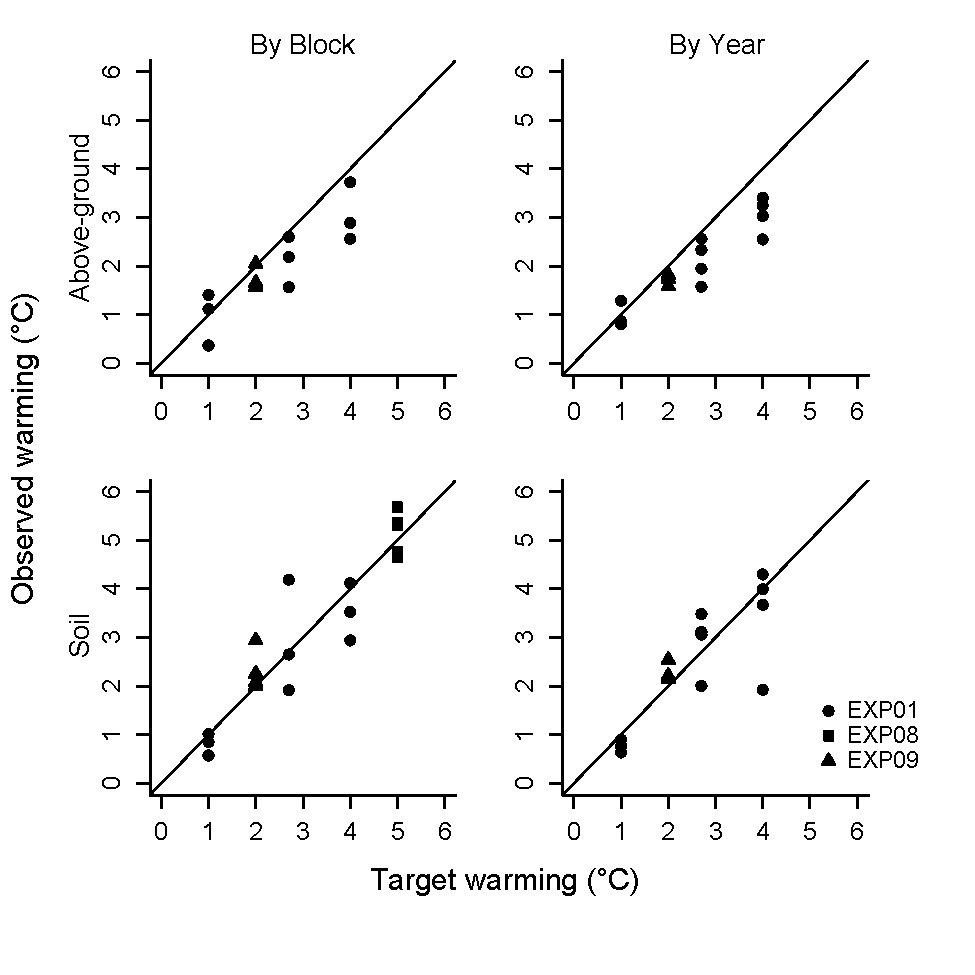
\includegraphics{../figures/BothWarmingbyblockyear.pdf}    
 \caption{The amount of warming (i.e. the difference between treatment and control plots, within each block) varies among blocks (left panels), as well as among years (right panels). See Tables 1 and 2 for statistical differences.} %EMW: line is 1:1? Also, we should have a map of the sites somewhere? New Figure 1?
 %during the time of the whole experiment? or annual mean?
 \end{figure}
\clearpage
 \begin{figure}[h]
     \centering
 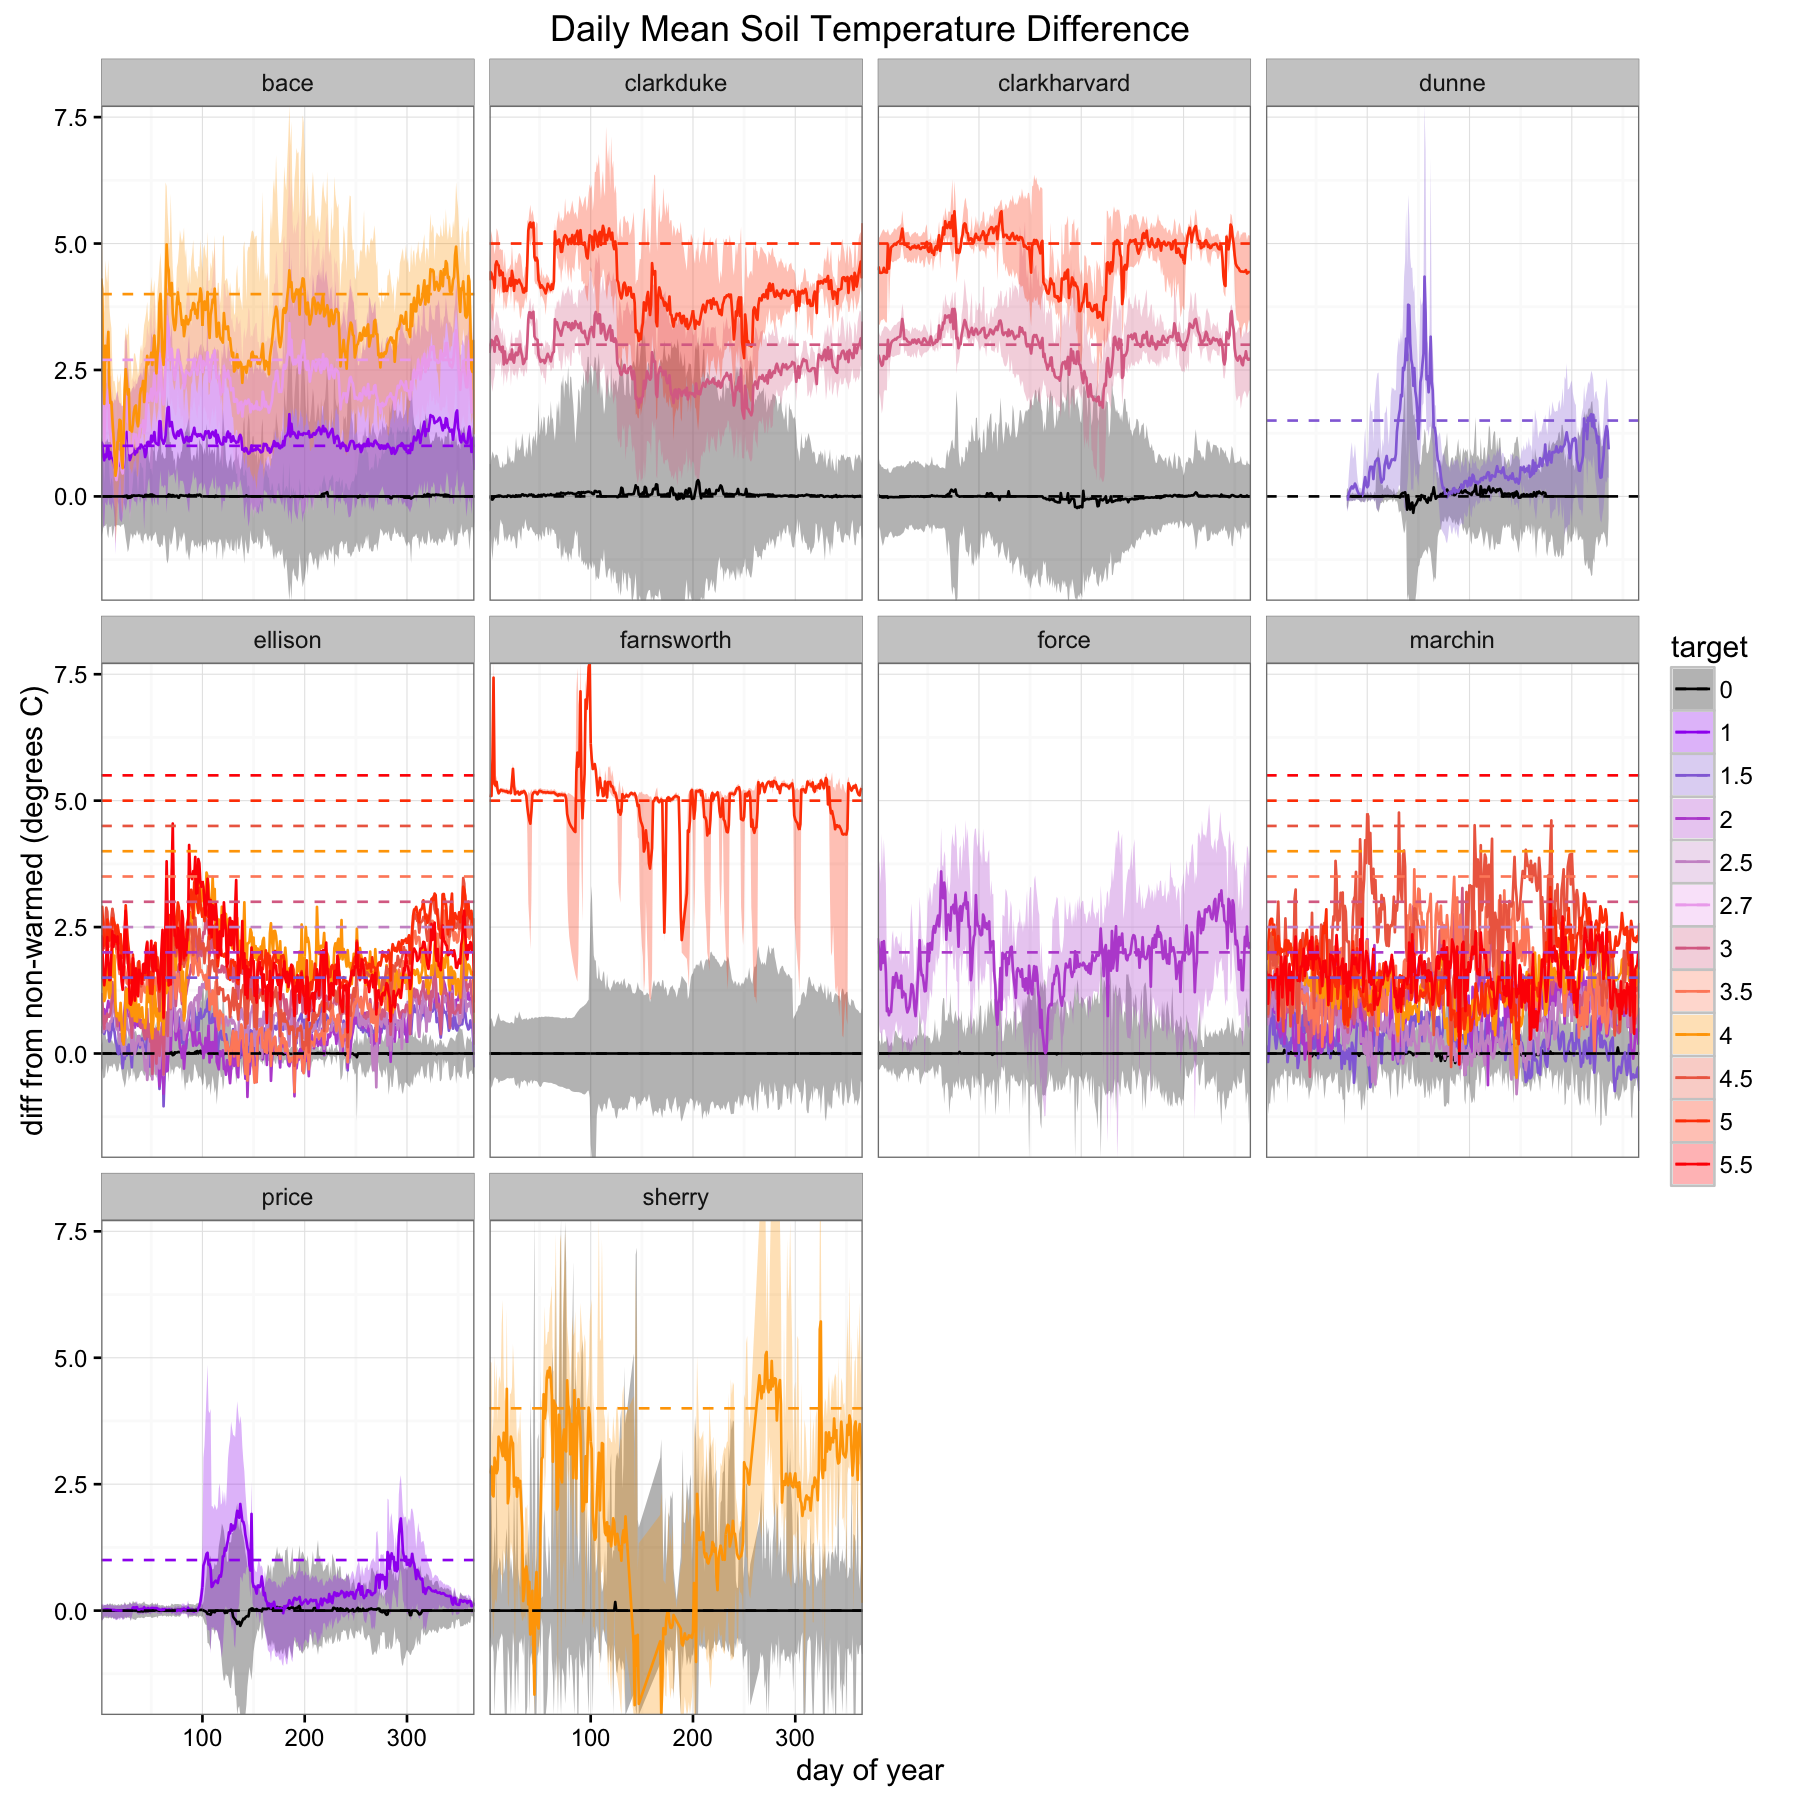
\includegraphics{../figures/Exploratory_TimeSeries_SoilTemp1Mean_Deviation.png}    
 \caption{Time series of deviations from mean soil temperature over one year, in control (black line) and warming treatments with various target warming levels at 10 study sites.} %EMW: This figure is great -- you should make it sound more exciting when you mention it in the main text.Yann: can you explain why we have such huge standard deviation for a given treatment or even in the control
 \end{figure}
\clearpage
 \begin{figure}[h]
     \centering
 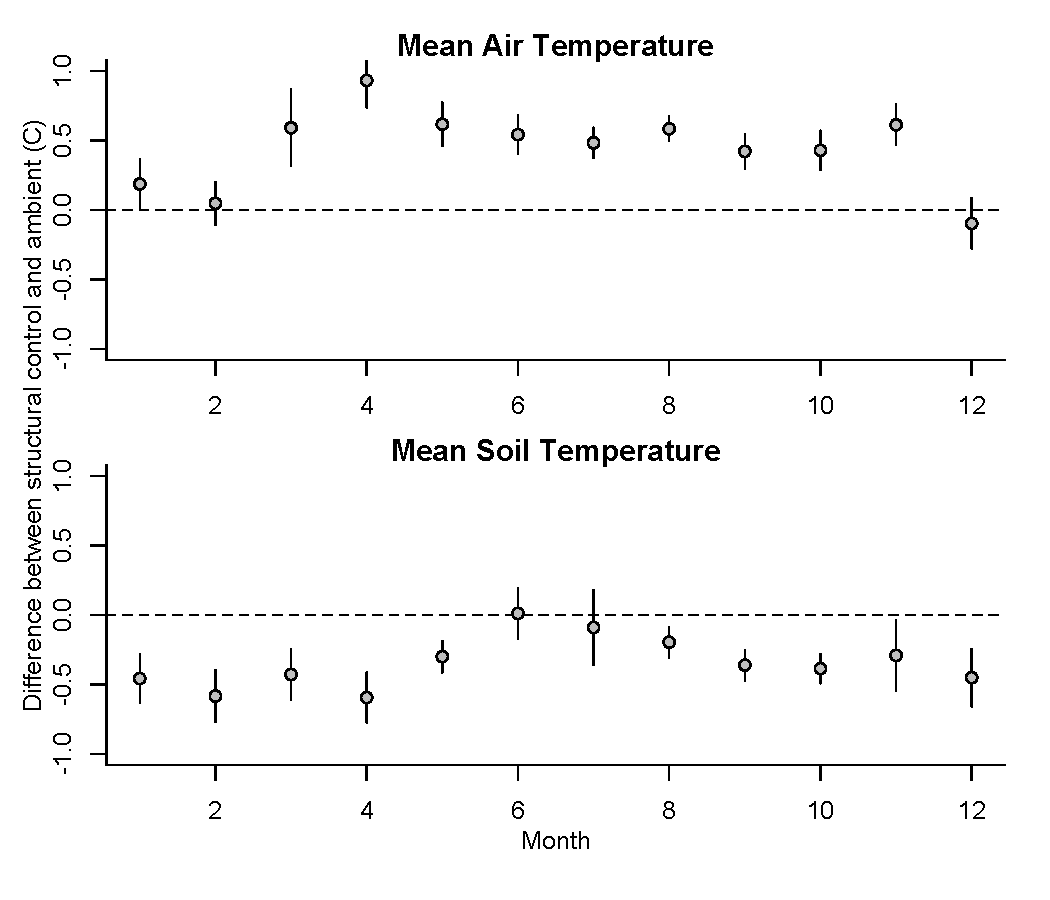
\includegraphics{../figures/ShamVSAmbient_mean.pdf}    
 \caption{Difference between mean air and soil temperatures in structural controls compared with ambient controls, with no control chambers or warming infrastructure in place. Air temperatures were higher, whereas soil temperatures were lower in the structural controls compared with ambient conditions. We show fixed effects from a mixed effects model that accounts for differences in experimental design and other factors among sites by including site as an intercept-only random effect (see Supplemental Materials for details). } %Ben: Is there significant snow at these sites during the winter? I wonder if the soil temperature difference could be a result of the shams interfering with the developing of an insulating layer of snow on the ground (which would normally keep the soils warmer). At any rate-great figure and another important detail to highlight.
 % Add ref to table in supp for stats.
 \end{figure}
 \clearpage
 \begin{figure}[h]
     \centering
 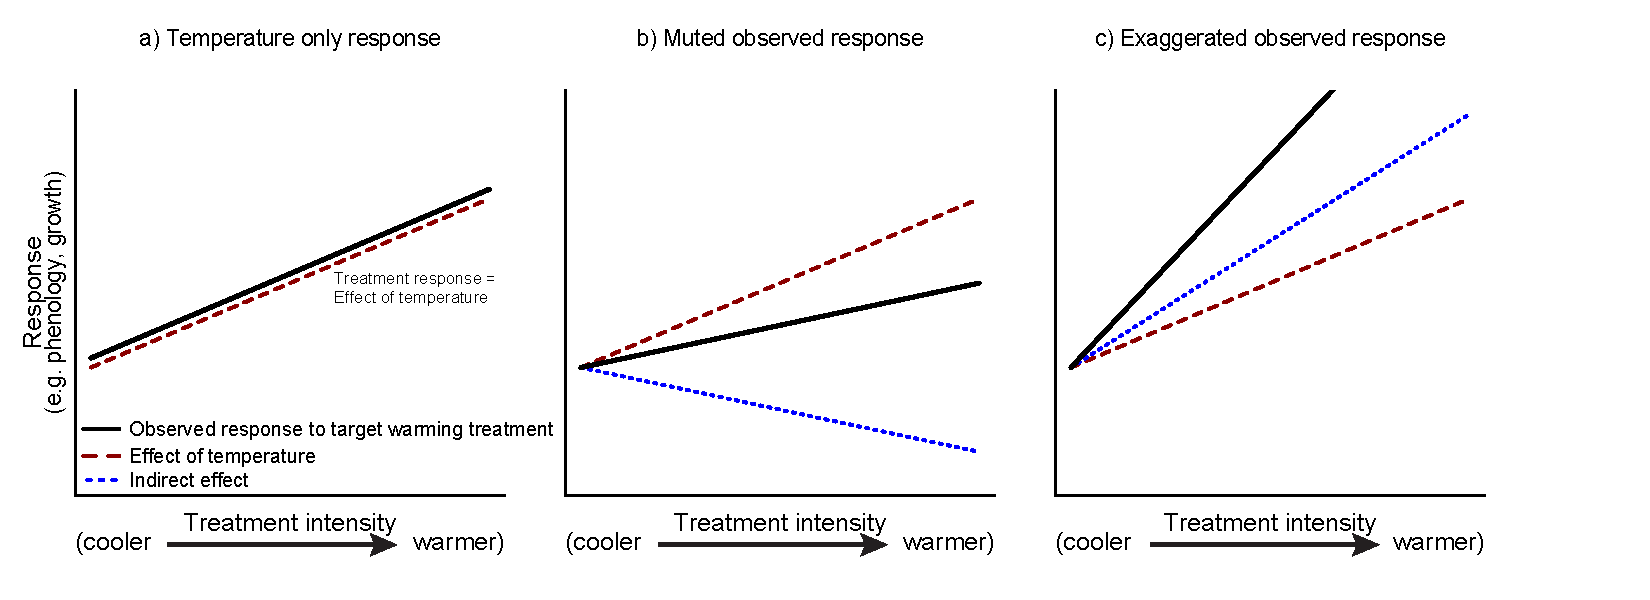
\includegraphics{../figures/DirIndWarmingEffects.pdf}    
 \caption{Experimental warming may cause biological responses to be muted or exaggerated, compared to direct responses to temperature alone, when indirect effects of experimental warming are also drivers of focal responses. For example, phenology may appear to be less sensitive to warming in experiments versus observational studies \citep{wolkovich2012} because experimental warming reduces soil moisture, perhaps more than natural warming.} 
 % EMW: Change the Y axis title so it's clearer -- effect of structural control (difference ....)? 
 % EMW: Explain phenology better (advances and delays) or just refer reader to main text for examples.
 \end{figure}
\clearpage
\section*{Supplemental Materials}
\subsection*{Description of database}
Search terms used and criteria for selecting the 12 studies that we ended up with. Climate variables included, and where database and metadata are housed.
\subsection*{Supplemental Methods}
\par\textit{Statistical methods}
\par Need description of block and year analyses (see Tables 1 and 2) 
To account for differences in the type of warming and other unmeasured site/study differences (e.g. forced air for Ellison and Marchin; heating cables for Farnsworth and ??), we fit linear mixed effects models with random effect of study-site. Response variables were daily soil or air temperature (models with daily  mean, minimum, and maximum were all fit) and , and the explanatory variable was control type (infrastructure or ambient). We used a random intercepts structure, so that the mean temperature was allowed to vary across study-sites. We fit models across the entire year, as well as separate models for each month to examine if effects varied seasonally.
%%%%%%%%%%%%%%%%%%%%%%%%%%%%%%%%%%%%%%%%
\end{document}
%%%%%%%%%%%%%%%%%%%%%%%%%%%%%%%%%%%%%%%%
